\section{Farmaci antipsicotici}

I \textbf{\emph{farmaci antipsicotici}} sono composti ampiamente
utilizzati in ambito psichiatrico per il trattamento dei disturbi
psicotici in una grande varietà di condizioni, tra cui vanno annoverate:

\begin{itemize}
\item
  la \emph{schizofrenia},
\item
  il \emph{disturbo} \emph{bipolare},
\item
  la \emph{depressione con manifestazioni psicotiche},
\item
  la \emph{psicosi farmaco-indotta} e quella \emph{senile}.
\end{itemize}

Questi farmaci, inoltre, possono avere anche degli effetti miglioranti
l'umore e possono ridurre l'ansia ed i disturbi del sonno, sebbene non
siano il trattamento di prima scelta quando questi sintomi costituiscono
il disturbo principale in pazienti non psicotici.
\\\\
Dal punto di vista strutturale, tipica degli antipsicotici è la
\textbf{struttura triciclica}, con tre anelli benzenici, che conferisce
un certo grado di attività anti-dopaminergica, comune a tutti gli
antipsicotici, anche se tale azione recettoriale varia notevolmente da
farmaco a farmaco (ad esempio la sulpiride ha quasi solo azione anti-D2,
mentre la clozapina ha uno spettro d'azione molto diversa, agendo
prevalentemente sui recettori 5-HT\textsubscript{2} piuttosto che sui
D2).
\\\\
In generale, gli antipsicotici possono essere suddivisi in:

\begin{itemize}
\item
  \textbf{\emph{tipici}} (sono per lo più \emph{bloccanti dei recettori
  D2}, anche se possono avere effetti anche su altri tipi di recettori)
\item
  \textbf{\emph{atipici}} (di più recente sviluppo, con \emph{prevalente
  blocco 5-HT\textsubscript{2}} piuttosto che D2).
\end{itemize}

\begin{figure}[!ht]
\centering
	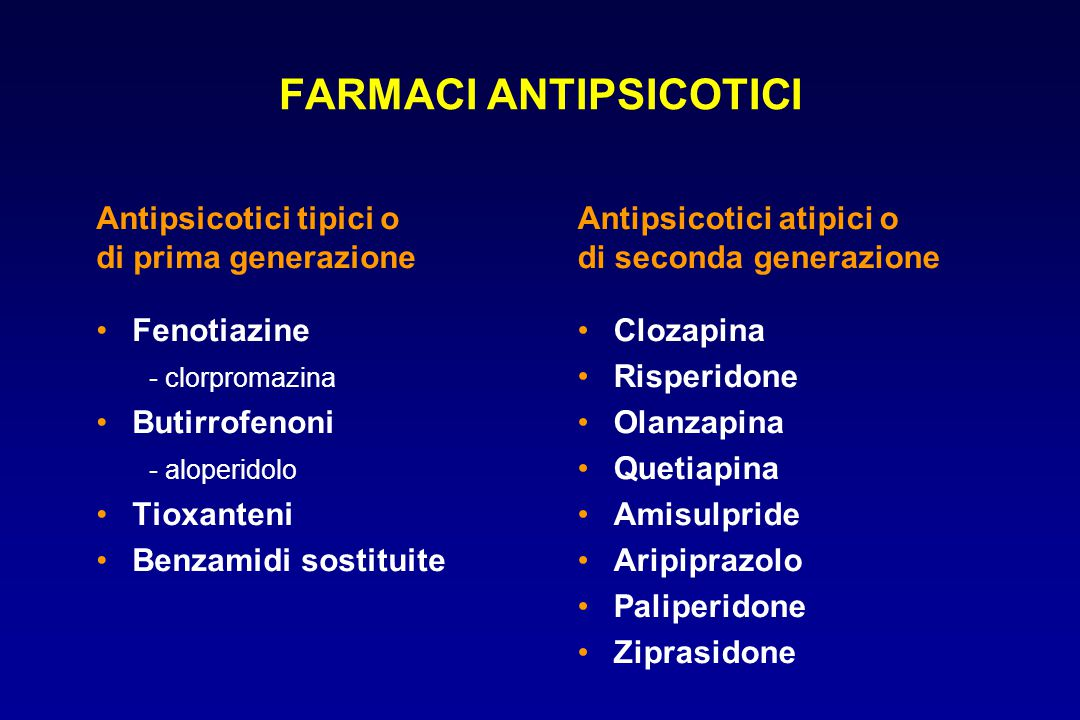
\includegraphics[width=0.9\textwidth]{07/image1.jpeg}
\end{figure}

\subsection{Trattamento della schizofrenia}

\subsubsection{Introduzione}

Possiamo raffigurarci la schizofrenia come un treno che investe la
persona che ne è affetta. L'idea rende perché effettivamente fermare un
treno in corsa non è una delle cose più semplici che si riesce a fare,
così come ad oggi non si riesce a guarire i pazienti affetti da questa
patologia: pensando al treno, riusciamo più che altro ad indirizzarlo.

A differenza di quanto detto sulla depressione e il disturbo bipolare la
schizofrenia è una malattia ad andamento cronico.

Per quanto riguarda le due precedenti patologie il problema principale è
che si riesce a trattare l'episodio acuto ma non c'è garanzia di evitare
le ricadute. Qui invece si può ottenere un miglioramento ma non una
remissione completa dei sintomi, quindi l'ottica è completamente
diversa.

L'esito previsto per questi pazienti è quindi ottenere il massimo
possibile alle condizioni permesse da questo disturbo.
\\\\
Il trattamento della schizofrenia ha come punto cardine l'utilizzo dei
\textbf{farmaci antipsicotici}, per cui è essenzialmente una
\textbf{\emph{farmacoterapia}}, ma un piano terapeutico appropriato
dovrebbe includere anche approcci psicoterapeutici, psicosociali e
riabilitativi, stabiliti di volta in volta in base alla risposta e a
progressi del paziente stesso. Nelle forme di schizofrenia catatonica,
inoltre, si può ricorrere anche all'uso della \textbf{\emph{terapia
elettroconvulsivante}}.

\begin{itemize}
\item
  \textbf{\emph{Trattamento Farmacologico}}

A tutt'oggi il trattamento di prime linea per la schizofrenia è quello
farmacologico, e si avvale essenzialmente degli \emph{antipsicotici},
suddivisi in \textbf{tipici} (noti anche come neurolettici, o
tranquillanti maggiori, che sono dei bloccanti dei recettori
D\textsubscript{2}) e \textbf{atipici} (di più recente sviluppo, sono
degli inibitori dei recettori 5-HT\textsubscript{2} ).

\begin{itemize}
\item[1.]
  Gli \textbf{\emph{antipsicotici tipici}} agiscono principalmente a
  livello della via dopaminergica mesolimbica, la cui iperattività si
  presuppone sia alla base dei \emph{sintomi positivi}, che
  effettivamente rispondono in genere bene agli antipsicotici tipici, i
  quali, dal punto di vista farmacodinamico, possono essere suddivisi
  in:

\begin{itemize}
\item
  \textbf{composti a bassa potenza} (\emph{tioridarina} e
  \emph{clorpromaziza}),
\item
  \textbf{ad alta potenza} (\emph{aloperidolo}, \emph{flufenazina}) in
  base all'affinità di legame coi recettori dopaminergici.
\end{itemize}

\item[2.]
  Gli \textbf{\emph{antipsicotici atipici}}, invece, si differenziano
  dai neurolettici per il loro diverso profilo clinico e tossicologico,
  ed hanno anche una maggior specificità d'azione nei confronti dei
  \emph{sintomi negativi}, potendo agire anche in soggetti che si sono
  precedentemente rivelati resistenti ai neurolettici.

  Gli antipsicotici atipici, inoltre, visto che non interagiscono con la
  trasmissione dopaminergica, \emph{non danno gli effetti collaterali di
  tipo extrapiramidale} tipici degli antipsicotici tipici, e risultano
  quindi meglio tollerati, garantendo una maggior compliance da parte
  del paziente.
\end{itemize}

Il trattamento farmacologico della schizofrenia è strutturato in 3 fasi
principali:

\begin{itemize}
\item
  \textbf{Fase Acuta}, che è volta al \emph{controllo dei sintomi
  dell'episodio psicotico acuto}, e che ha una durata media di \emph{6-8
  settimane};
\item
  \textbf{Fase di Stabilizzazione}, che consente nel \emph{proseguimento
  della cura a dosi piene per almeno 6 mesi}, così da consolidare i
  risultati ottenuti;
\item
  \textbf{Fase di Mantenimento}, finalizzata alla \emph{profilassi delle
  ricadute e la cui durata varia da 1 a 5 anni o più}.
\end{itemize}

\textbf{Fase Acuta}: In genere nella fase acuta si utilizzano dei
\textbf{neurolettici ad elevata potenza}, come l'\emph{aloperidolo} a
dosi di 10-15 mg/die, oppure si possono usare degli
\textbf{antipsicotici atipici}, come il \emph{risperidone} (4-6 mg/die),
l'\emph{olanzapina} (10-20 mg/die) o la \emph{quetiapina} (400-800
mg/die).
\\\\
Negli ultimi anni, le linee guida internazionali hanno preso a
raccomandare gli antipsicotici atipici come farmaco di prima scelta per
le fasi acute, sia come alternative ai neurolettici in pazienti con
suscettibilità a sviluppare effetti collaterali gravi o intollerabili.
\\\\
Se dopo 3 settimane di trattamento il paziente mostra una risposta
parziale è opportuno proseguire la cura, eventualmente aumentando le
dosi, per altre 6 settimane prima di cambiare il farmaco, mentre è bene
sostituirlo subito se non si ha un miglioramento apprezzabile dopo 2
settimane.
\\\\
Nei pazienti con \emph{elevata componente ansiosa ed agitazione
psicomotoria} è invece opportuno \emph{associare un neurolettico a bassa
potenza} (ad esempio la clorpromazina 100-300 mg/die) ad una
\emph{benzodiazepina} (lorazepam 7,5-12,5 mg/die).
\\\\
Si definiscono propriamente ``\textbf{resistenti}'' alla terapia quei
pazienti che hanno portato a termine almeno tre periodi di trattamento
negli ultimi 5 anni con tre antipsicotici diversi, appartenenti a due
classi chimiche diverse, con almeno 6 settimane a dosaggio adeguato, e
senza una scomparsa dei sintomi. In questi casi è opportuno passare alla
\textbf{\emph{clozapina}}, l'antipsicotico più efficace al momento
disponibile, il cui uso deve però essere attentamente controllato,
perché il farmaco può causare un'agranulocitosi potenzialmente letale
nell'1-2\% dei pazienti.
\\\\
Altre strategie per la fase acuta consistono nell'\emph{associazione di
antipsicotici e stabilizzanti dell'umore o benzodiazepine}, anche se
l'efficacia di tali terapie farmacologiche di associazione non è stata
ancora valutata nei dettagli. In caso di comparsa di sintomi
extrapiramidali, più comuni con i neurolettici, si può tentare ad
aggiungere un \textbf{farmaco anticolinergico} (orfenadrina 50-150
mg/die, oppure triesifenidile 2-6 mg/die), mentre se il sintomi
predominante è l'acatisia è utile l'aggiunta di un \textbf{$\beta$-bloccante}.
\\\\
\textbf{Fase di Stabilizzazione}: Consiste nel \emph{proseguimento della
terapia prescritta per la fase acuta}, avendo cura di adattarlo, se
necessario, alle condizioni del paziente tramite aggiunta di farmaci di
associazioni o modificando leggermente le dosi.
\\\\
\textbf{Fase di Mantenimento}: Una volta raggiunta la stabilità nei
sintomi è necessario formulare un programma terapeutico a lungo termine,
che includa trattamenti farmacologici, psicoterapeutici ed interventi di
tipo riabilitativo psicosociale, così da prevenire le ricadute e
migliorare la qualità della vita.

\item
  \textbf{\emph{Terapia Elettroconvulsivante}}

L'impiego della \textbf{terapia} \textbf{elettroconvulsivante}
(\textbf{TEC}) è ad oggi limitato ai casi in cui è presente una marcata
componente affettiva (depressione secondaria o disturbo
schizoaffettivo), nelle forme catatoniche e, in associazione ai farmaci,
nei casi resistenti al solo trattamento farmacologico.

\end{itemize}

\subsubsection{Evoluzione della terapia}

\begin{figure}[!ht]
\centering
	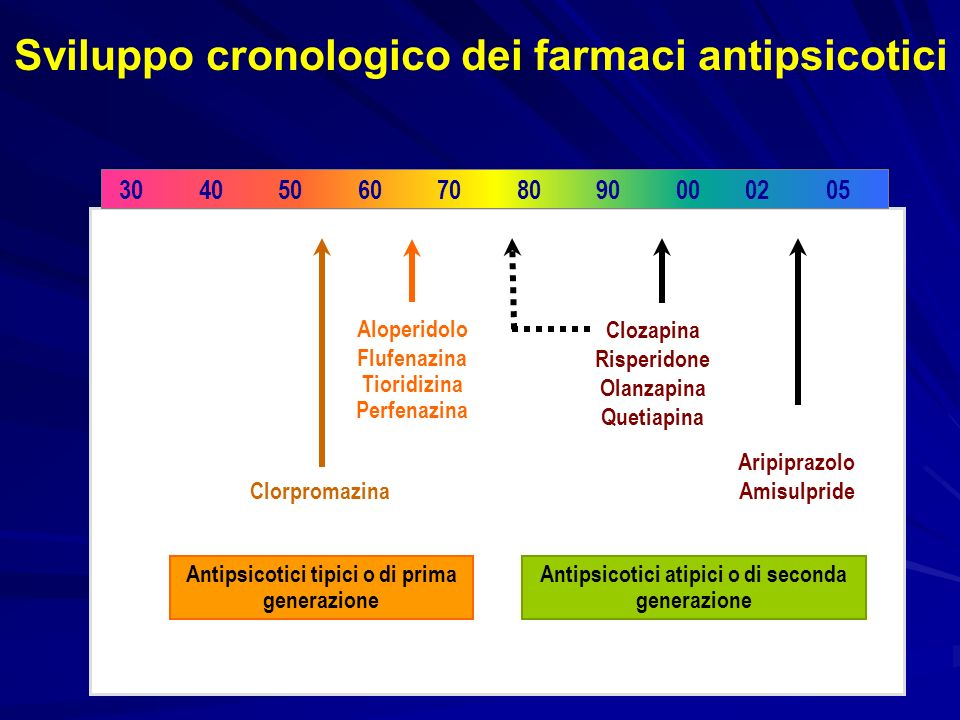
\includegraphics[width=0.9\textwidth]{07/image2.jpeg}
\end{figure}

Dal punto di vista storico, i primi studi sugli antipsicotici risalgono
agli \textbf{anni '60}, quando nel 1952 in Francia si vide che la
\textbf{clorpromazina}, un farmaco usato come ipotermizzante negli
interventi chirurgici, si rivelò dotata di una buona azione
antipsicotica, e a seguito di tale scoperta vennero poi identificate
anche altre molecole ad azione analoga, che vennero generalmente
indicate come \emph{neurolettici.}

I farmaci antipsicotici fin qui scoperti, detti in seguito
\textbf{\emph{antipsicotici tipici}}, si rivelarono in effetti efficaci
nel trattamento dei sintomi positivi, ma erano molto meno efficaci nel
trattamento di quelli negativi, nei confronti dei quali si rivelarono
molto utili altri composti, successivamente denominati
\textbf{\emph{antipsicotici atipici}}, il cui prototipo era la
\textbf{clozapina}, un farmaco scoperto già negli \textbf{anni '70}, ma
che era stata abbandonata nel momento in cui era apparso il suo
principale effetto collaterale, una grave forma di agranulocitosi
potenzialmente mortale.

Sul \textbf{finire degli anni '80} si è visto che in un 30\% dei
pazienti il blocco dei soli recettori D2 non aveva alcun effetto e
risultavano insensibili alla terapia nonostante si aumentassero le dosi
(es. dosi di Aloperidolo da 300 mg/die su un range normale di 4 -- 20
mg): l'unica evidenza era un peggioramento degli effetti collaterali.

Due farmacologi clinici americani iniziarono quindi a sperimentare sui
pazienti \emph{non responders} ad una dose di farmaco per un totale
equivalente di 1000 mg di Clorpromazina in 6 settimane (cioè la dose
totale assunta in questo lasso di tempo). Crearono due farmaci di classe
chimica differente

\begin{itemize}
\item
  Fenotiazine
\item
  Butirrofenoni
\end{itemize}

Non risposero comunque, mantenendo un punteggio elevato nella scala di
sintomatologia che era stata creata. Dopodichè si è provato a testarli
con un 60 mg di Aloperidolo per 6 settimane. Migliorava il 4\% di quelli
trattati con Clorpromazina, mentre il 20\% di quelli trattati con
l'Aloperidolo.

\textbf{All'inizio degli anni '90} riemerge la Clozapina proprio perché
avendo un'attività a così ampio spettro riusciva ad essere efficace nei
pazienti in cui nient'altro funzionava, era efficace nel trattamento di
quelle forme psicotiche che erano invece refrattarie alla terapia con
altri composti tipici. Per tali motivi, ed anche per il fatto che il
rischio relativo di agranulocitosi nella popolazione europea fu stimata
attorno allo 0,7\% (più alta nei soggetti provenienti dal Nord Europa),
si decide si consentire l'uso della clozapina nel trattamento dei
disturbi psicotici, ponendo però come precauzione un esame
emocromocitometrico ogni settimana nei primi 4 mesi, poi una volta al
mese.

La pubblicità di questo farmaco era \emph{``Jack is back''} con
l'immagine di Jack che tornava a lavorare.

La realtà non è proprio così, nel senso che l'efficacia era di avere un
qualche tipo di effetto dove nient'altro aveva funzionato: si sa che
questo non coincide con la guarigione.

\textbf{Nei primi anni 2000,} infine, sono stati scoperti altri farmaci
antipsicotici atipici, oggi definiti ``\textbf{\emph{di seconda
generazione}}'', i quali, come la \textbf{clozapina}, danno generalmente
\emph{minori effetti extrapiramidali}, danno un \emph{minor aumento
della concentrazione della prolattina} ed agiscono principalmente da
\emph{antagonisti dei recettori 5-HT\textsubscript{2}},ad esempio il
\textbf{risperidone} \emph{,}l'\textbf{amilsulipiride},
l'\textbf{aripiprazolo}.
\\\\
Un problema di questa evoluzione farmacologica sono stati i costi,
perché da un costo medio di 50 dollari all'anno per un paziente trattato
con aloperidolo si è passati ai 9000 per la Clozapina, a cui si
aggiungevano gli emocromi tutte le settimane per le prime 48.

L'Olanzapina non dà agranulocitosi e aveva un costo di 6500 dollari
l'anno.

E' giustificato spendere tanto di più se un farmaco ci dà di più. Mentre
per la Clozapina non ci sono dubbi, per gli altri la situazione è da
valutare tant'è che nel 2000 uscì un editoriale sul British Medical
Journal dal titolo ``il gioco non vale la candela''.

Ad oggi uno studio riporta i risultati dell'efficacia del trattamento di
5 farmaci diversi, di prima e di seconda generazione: la prima cosa che
emerge è che si ottiene lo stesso miglioramento con tutti i farmaci
(Clozapina esclusa).

\emph{\textbf{Efficacy}}: risultati ottenuti tramite Clinical Trial, con
controlli elevati

\emph{\textbf{Effectivness}}: dati ottenuti dalla pratica clinica in
condizioni sperimentali meno controllate ma comunque indicative.

\paragraph{Antipsicotici tipici ("neurolettici")}

Gli \textbf{\emph{antipsicotici tipici}} sono noti anche come
\emph{tranquillanti maggiori} o \emph{neurolettici} a causa dell'effetto
collaterale da blocco dopaminergico che si manifesta con tremori e
sintomi extrapiramidali.

Quindi il termine ``neurolettico'' è stato dato perché questi farmaci
avevano la funzione di ridurre l'attività neuronale, non scevri però da
effetti collaterali.

Inizialmente l'Indicazione terapeutica era somministrare e aumentare le
dosi del farmaco finché non si manifestavano i tipici effetti
collaterali, quali tremore e ipotensione, sintomi extrapiramidali etc.
Questo significa che l'attività terapeutica diventava inscindibile
dall'effetto collaterale.

\emph{\emph{Classificazione:}}

Questi composti possono inoltre essere suddivise in diverse classi
chimiche, tra cui bisogna ricordare le principali:

\begin{itemize}
\item
  \textbf{Fenotiazine}, a loro volta suddivise in \emph{fenotiazine
  alifatiche} (clorpromazina), \emph{fenotiazine piperidiniche}
  (tioridazina) e \emph{fenotiazine piperaziniche} (flufenazina);
\item
  \textbf{Butirrofenoni}, rappresentati essenzialmente dall'aloperidolo;
\item
  \textbf{Tioxanteni}, come il tiotixene;
\item
  \textbf{Dibenzoxazepine}, come la loxapina.
\end{itemize}

\emph{\emph{Usi clinici:}}

Indipendentemente dalla classe chimica di appartenenza, tutti questi
composti sono efficaci soprattutto sui \emph{sintomi positivi}, mentre
quelli negativi permangono inalterati o possono addirittura peggiorare,
così come possono peggiorare anche i sintomi cognitivi, infatti si
possono riscontrare problemi di memoria immediata e pratica, nonché
delle funzioni cognitive, dell'attenzione e della concentrazione.

Gli antipsicotici tipici, in ogni caso, esercitano un \emph{effetto
antipsicotico}, \emph{sedativo} e \emph{disinibente}, utile soprattutto
nelle manifestazioni autistiche.

\emph{\emph{Profilo molecolare:}}

L'azione comune è il \textbf{blocco dei recettori D2}, che ha portato
evidenze a supporto dell'ipotesi dopaminergica della schizofrenia, e
l'effetto terapeutico si spiega mediante il blocco dei circuiti
mesocorticali e mesolimbiche.

\emph{\emph{Effetti collaterali:}}

L'inevitabile azione anche su:

\begin{itemize}
\item
  \textbf{via tubero-infundibulare} causa \emph{amenorrea} e
  \emph{disfunzioni sessuali} (infatti la dopamina, tramite i sui
  recettori D2, ha un'azione inibitoria nei confronti del rilascio della
  prolattina a livello ipofisario),
\item
  mentre il blocco dopaminergico a \textbf{livello nigro-striatale}
  determina la comparsa degli \emph{effetti extrapiramidali}, che sono
  particolarmente marcati proprio con gli antipsicotici tipici e
  includono:

\begin{itemize}
\item
  effetti acuti come:

\begin{itemize}
\item
  le \textbf{distonie} a livello del tronco e degli arti, che richiedono
  l'aggiunta di farmaci anticolinergici,
\item
  \textbf{crisi a livello oro-linguale}, che possono dare anche
  contratture molto dolorose, così come torsione dei bulbi oculari verso
  l'alto, e tutte queste manifestazioni acute in genere compaiono entro
  5 giorni dall'inizio del trattamento nel 40-60\% dei pazienti.
\end{itemize}

\item
  Altre forme ad esordio più tardivo sono: il \textbf{parkinsonismo},
  che compare in genere dopo 3-4 mesi, e l'\textbf{acatisia}, che è
  dipendente dal blocco nigro-striatale e consiste nell'impossibilità a
  stare fermi o in una marcata irritabilità, le \textbf{discinesie}
  (\emph{Rabbit Syndrome}: è un tipo particolare di discinesia che imita
  il movimento di masticazione del coniglio), i \textbf{tremori.}

  Per ovviare a parkinsonismo e discinesie, spesso tardive (dopo
  settimane o mesi di trattamento) si proponevano le cosiddette
  \emph{\textbf{drug holidays}}, cioè una sospensione del farmaco
  temporanea proprio per attenuare queste manifestazioni. Se non era il
  medico a prescriverle erano comunque i pazienti stessi perché la
  situazione diventava ingestibile. Il problema era che deliri e
  allucinazioni ricomparivano molto rapidamente, con un tasso di
  ricaduta del 10\% che aumentava di mese in mese.
\end{itemize}

\item
  il forte \textbf{blocco sui recettori $\alpha$\textsubscript{1}, M1 ed H1}
  determina gli effetti collaterali più frequenti, come \emph{nausea},
  \emph{vomito}, \emph{ipotensione ortostatica}, \emph{sedazione} ed
  \emph{incremento dell'intake di cibo}.
\item
  La \textbf{scarsa azione sui recettori 5-HT\textsubscript{2}}
  giustifica l'inefficacia di questi farmaci nei confronti dei sintomi
  negativi,
\end{itemize}

\emph{\emph{Capostipite:}}

Il capostipite degli antipsicotici tipici è
l'\textbf{\emph{aloperidolo}}, un potente bloccante dei recettori D2
mesocorticali e un poco attivo anche sui recettori
5-HT\textsubscript{2A} e 5-HT\textsubscript{1A}, oltre al consueto
blocco sui recettori $\alpha$\textsubscript{1}, M1 ed H1.
\\\\
Accanto alla classe dei neurolettici vennero poi proposte anche altre
classi farmacologiche, come quella dei cosiddetti \emph{farmaci
incisivi} (che agivano cioè prevalentemente sui sintomi positivi), i
\emph{farmaci sedativi} (usati per l'effetto tranquillante) ed i
\emph{farmaci ad azione disinibente}, cioè che cercavano di contrastare
l'isolamento del paziente, ma oggi questa tutte queste distinzioni sono
state abolite, preferendo basarsi solo sul profilo d'azione molecolare
del composto e della classe chimica a cui appartiene.

Sino agli '70-'80 non era ancora ben chiaro il meccanismo d'azione dei
farmaci antipsicotici, che divenne poi chiaro risiedere
nell'\textbf{\emph{antagonismo dei recettori D2}}, per cui nei primi
periodi furono proposte diverse terapie di associazione, in cui si
cercava di combinare (in genere senza risultati soddisfacenti) più
antipsicotici diversi, nella speranza di ottenere risultati migliori a
fronte di effetti collaterali minori. Dalla fine degli anni '80, e poi
decisamente dai primi anni '90, si scelse si sostituire il termine
``neurolettico'' con ``\emph{antipsicotico}'', così da separare, almeno
dal punto di vista semantico, l'effetto terapeutico da quello
collaterale

\paragraph{Antipsicotici atipici}

Col tempo si è cercato di scindere l'effetto terapeutico da quello
collaterale e quindi si è preferito il termine antipsicotici a quello
neurolettici per indicare il cambio d'indirizzo terapeutico, ottenuto a
partire dagli anni '90 con quelli di 2\textsuperscript{o} generazione. Si cercò di mettere
a punto farmaci con minori effetti collaterali, che non rendevano più
necessario cercare l'effetto collaterale per capire l'efficacia del
farmaco, e questo perché si comprese che l'effetto farmacologico
desiderato compariva quando venivano bloccati circa i \emph{2/3 dei
recettori D2} presenti a livello cerebrale, e al di sopra di tale valore
oltre all'effetto farmacologico comparivano gli effetti extrapiramidali,
per cui si riuscì finalmente a stabilire un dosaggio più preciso ed
efficace, capace di bloccare esattamente il 65-70\% circa dei recettori
D2, abbandonando le dosi eccessivamente elevate che avevano
caratterizzato il periodo precedente.

Gli \textbf{\emph{antipsicotici atipici}}, dimostrarono un'efficacia
anche nei confronti dei \emph{sintomi negativi} e creano minori
problematiche di natura cognitiva e minori effetti collaterali.

\emph{\emph{Classificazione: }}

Dal punto di vista chimico, gli antipsicotici atipici appartengono alla
classe:

\begin{itemize}
\item
  delle \textbf{dibenzoazepine} (come la clozapina),
\item
  dei \textbf{benzisossazoli} (come il risperidone)
\item
  delle \textbf{tienobenzodiazepine} (come l'olanzapina).
\end{itemize}

\emph{\emph{Capostipite:}}

Il capostipite degli antipsicotici atipici, nonché il farmaco più
efficace di tutta la categoria, che agisce soprattutto tramite un blocco
sui recettori 5-HT\textsubscript{2A}, soprattutto in sede prefrontale, è
la \textbf{\emph{clozapina}}.

\emph{\emph{Effetti collaterali di Clozapina:}}

Gli antipsicotici atipici hanno minori effetti collaterali
extrapiramidali per via del \emph{ridotto effetto di blocco
dopaminergico}, ma conservano tuttavia i loro effetti sui
\emph{recettori $\alpha$\textsubscript{1}, M1 ed H1.}

Gli effetti collaterali della clozapina includono:

\begin{itemize}
\item
  un'\textbf{agranulocitosi} che si caratterizza per \emph{neutropenia}
  (neutrofili al di sotto delle 500 unità/mm\textsuperscript{3}) e
  \emph{leucopenia} (con leucociti al di sotto delle 3500
  unità/mm\textsuperscript{3}).

  A tutt'ora il rischio di questa complicazione ha una probabilità
  stimata attorno allo \textbf{0,7\%}, (prima era del 2\% circa). Questo
  rischio impone di \emph{fare settimanalmente un emocromo}, almeno nei
  primi 4 mesi di terapia, e nel momento in cui si osservasse la
  neutropenia si deve immediatamente sospendere il farmaco, e così
  facendo la percentuale di sviluppo di agranulocitosi grave è
  sovrapponibile a quella di qualsiasi altro antipsicotico.

  Come regola generale questo farmaco è per definizione di seconda
  scelta, da usare solo per forme gravi e resistenti agli altri
  antipsicotici, e la si usa in pazienti non responders che abbiano già
  provato con almeno due altri farmaci appartenenti a classi
  farmacologiche diverse.

  Il problema dell'agranulocitosi, peraltro, è un \emph{disturbo su base
  immunitaria}, ed è quindi un grave problema, perché anche se si prova
  a somministrarla anche a distanza di tempo il problema si ripresenta,
  anzi tende ad aumentare sempre più.

  Fattori di rischio per lo sviluppo di questo effetto collaterale sono
  l'\emph{età avanzata}, il \emph{sesso} \emph{femminile}, una certa
  \emph{predisposizione genetica} e possibili \emph{fattori tossici o
  autoimmuni}.

  N:B: Una cosa da tenere sempre a mente, tuttavia, è che non si deve
  \textbf{\emph{mai associare la clozapina col litio}}, che già di per
  sé può causare una leucocitosi, tanto che si può avere una leucopenia
  inapparente nelle prime 2 settimane, ed alla terza settimana le
  conseguenze possono essere già molto gravi.
\item
  In virtù del \emph{blocco D2} a livello tubero-infundibulare, inoltre,
  si sviluppa \textbf{iperprolattinemia}, soprattutto a seguito di un
  precedente trattamento con \emph{risperidone} o \emph{amilsulpiride};
  questa iperprolattinemia è dose-dipendente:

  nelle donne causa tensione mammaria, galattorrea ed amenorrea,

  nei maschi causa sempre tensione mammaria, galattorrea, riduzione
  della libido, impotenza e ginecomastia, ma non ha effetti cancerogeni.
\item
  Il \emph{blocco dei recettori $\alpha$\textsubscript{1}}-adrenergici causa
  \textbf{ipotensione ortostatica},
\item
  L'azione di \emph{blocco dei recettori H1} dà \textbf{sedazione} e
  \textbf{incremento ponderale},
\item
  Il \emph{blocco sui recettori M1} dà \textbf{sintomi cognitivi}, come
  disturbi dell'attenzione, della concentrazione e della memoria, ma
  hanno effetti anche sull'apparato gastro-intestinale, come il
  \textbf{rallentamento della peristalsi}, con \textbf{stipsi}, nonché
  \textbf{secchezza delle} \textbf{fauci}, \textbf{glaucoma},
  \textbf{ipertrofia prostatica}, \textbf{tachicardia}.
\item
  Altri effetti collaterali legati alla clozapina sono l'\textbf{aumento
  delle transaminasi epatiche}, \textbf{scialorrea}, \textbf{aumentata
  sudorazione}
\item
  Ad alto dosaggio, \textbf{crisi convulsive}.
\item
  I \textbf{problemi a livello cardiologico} sono comuni a tutti gli
  antipsicotici, in particolare si può avere un \textbf{allungamento del
  tratto QT}, soprattutto con la clozapina ed alcuni nuovi composti,
  come la quetiapina, per cui è consigliato un monitoraggio con ECG
  all'inizio della terapia ed uno dopo 15 giorni con calcolo
  dell'eventuale variazione rispetto alla registrazione precedente.
  Fattori di rischio per l'allungamento del tratto QT sono il
  \emph{sesso femminile}, l'\emph{ipokaliemia} e le \emph{sindromi
  congenite del QT lungo}, dovute a mutazioni dei canali del
  K\textsuperscript{+} o del Na\textsuperscript{+}.
\item
  Una particolare manifestazione dovuta alla clozapina è poi la
  \textbf{\emph{sindrome maligna da neurolettici}}, che è causata anche
  da altri antipsicotici: l'evoluzione di questa condizione è mortale
  nel 20\% dei casi se non trattata, ma se è riconosciuta subito e
  trattata non ha complicanze gravi.

  La sindrome si manifesta nello 0,2-0,4\% dei pazienti trattati con
  antipsicotici, ed è più frequente con gli antipsicotici di I
  generazione e di elevata potenza, caratterizzandosi per:

\begin{itemize}
\item
  \emph{rialzo termico},
\item
  \emph{rigidità muscolare},
\item
  squilibrio del sistema neurovegetativo con \emph{tachicardia},
  \emph{tachipnea}, \emph{disfagia}, \emph{ipotensione},
  \emph{sudorazione profusa} e talvolta anche \emph{ipertensione
  diastolica}. I
\end{itemize}

Il paziente si presenta immobile, rigido, con una contrattura di tipo
spastico, in una condizione di stupore, ed è scarsamente reattivo,
talora confuso. La contrattura porta ad un incremento plasmatico di CPK,
delle transaminasi, dell'aldolasi, dell'LDH ed anche della mioglobina,
con conseguente \emph{mioglobinuria} ed \emph{insufficienza renale}.
\\\\
Questi pazienti devono essere trattati, essendo la patogenesi legata ad
un blocco dopaminergico a livello ipotalamico, con \textbf{agonisti
dopaminergici} come la \emph{bromotriptina} oppure, siccome prevale la
contrattura a livello periferico muscolare, con dei \textbf{chelanti del
calcio}, come il \emph{nantrolene sodico}, somministrato a dosi di 1-2
mg per via endovenosa, oltre al posizionamento di un sondino
naso-gastrico, perché questi pazienti non si alimentano spontaneamente.
È fondamentale diagnosticare questa sindrome per tempo, in quanto i
pazienti possono morire per insufficienza renale, TEP o per
insufficienza renale.
\end{itemize}

\emph{\emph{Altri antipsicotici atipici:}}

Nei primi anni 2000, infine, sono stati scoperti altri farmaci
antipsicotici atipici, oggi definiti ``\textbf{\emph{di seconda
generazione}}'', i quali, come la \textbf{clozapina}, danno generalmente
minori effetti extrapiramidali, danno un minor aumento della
concentrazione della prolattina ed agiscono principalmente da
\emph{antagonisti dei recettori 5-HT\textsubscript{2}}:

\begin{itemize}
\item
  il \textbf{risperidone} \emph{ad alte dosi può dare sintomi
  extrapiramidali rilevanti},
\item
  l'\textbf{amilsulipiride} \emph{blocca i recettori D2 piuttosto che i
  5-HT\textsubscript{2}}.
\item
  Caso particolare è rappresentato dall'\textbf{aripiprazolo},
  commercializzato col nome di Abilify, che è un \emph{agonista parziale
  dei recettori D2}, dai cui studi è emerso che la schizofrenia non sia
  dipendente solo da un aumento della dopamina, ma anche dalla presenza
  di un difetto localizzato corticale che funge da ``primus movens'' a
  livello mesolimbico e mesocorticale per l'aumento dopaminergico,
  quindi, almeno a livello teorico se si agisse con un farmaco, come un
  agonista parziale si potrebbe ottenere un miglior bilanciamento tra
  aree con minore e maggiore presenza di neurotrasmettitore rispetto al
  normale, anche se attualmente questo meccanismo farmacologico, sul
  piano clinico, si è rivelato poco efficace.
\end{itemize}

\paragraph{Farmacodinamica e farmacocinetica degli antipsicotici}

\emph{\emph{Farmacodinamica}}

Per quanto riguarda il profilo farmacodinamico degli antipsicotici, il
composto che sino ad oggi ha dimostrato un'\emph{efficacia maggiore è la
\textbf{clozapina}}, la quale tuttavia ha anche notevoli effetti
collaterali, per cui viene in genere riservata per disturbi psicotici
gravi e non responsivi ad altri farmaci, i quali hanno peraltro più o
meno lo stesso livello di efficacia. In realtà si deve precisare che
questi farmaci, anche se in grado diverso, funzionano sempre, infatti
nella fase acuta i pazienti migliorano nel 50-60\% dei casi e le
ricadute sono minori nel momento in cui il paziente viene trattato più a
lungo possibile con dosi basse. Per quanto riguarda invece la potenza,
essa viene espressa come la dose capace di determinare un certo effetto,
quindi a parità di effetto desiderato, a dosi minori corrisponde una
potenza maggiore rispetto ad un farmaco che ottiene il medesimo effetto
ma a dosi più elevate. L'\textbf{aloperidolo} è l'\emph{antipsicotico
con maggior potenza}, quindi è il più antidopaminergico, ma anche un
bloccante dei recettori H1 ed M1, per cui sulla base della potenza si
possono anche prevedere i possibili effetti collaterali.

\emph{\emph{Farmacocinetica:}}

Dal punto di vista farmacocinetico, alcuni antipsicotici hanno un
\emph{assorbimento rapido e completo}, come nel caso
dell'\textbf{aloperidolo}, per altri, come la \textbf{clorpromazina},
l'assorbimento è \emph{lento ed incompleto} se somministrata per via
orale. Ovviamente, se l'antipsicotico viene somministrato invece per via
parenterale la concentrazione efficace è raggiunta molto più
rapidamente, e gli effetti sedativi tendono anch'essi a manifestarsi più
precocemente, tanto che in passato si sfruttava tale fenomeno per
indurre una ``\emph{tranquillizzazione rapida}'' nei pazienti agitati.
Molto utili sono poi le ``\textbf{\emph{formulazioni depot}}'', cioè
somministrazioni di antipsicotico in veicolo oleoso, in modo da dare una
lenta liberazione del composto a partire dal sito di somministrazione,
garantendone così una concentrazione stabile in periodi relativamente
lunghi, e questa strategia viene tipicamente messa in atto in pazienti
poco complianti, che faticano ad assumere giornalmente l'antipsicotico
per via orale.

\paragraph{Profilo molecolare}

Dal punto di vista del profilo molecolare, tutti i farmaci
antipsicotici, ma in particolare i \textbf{\emph{neurolettici,}}
agiscono da \textbf{antagonisti recettoriali D2}, ma interagiscono anche
con altri tipi di recettori:

\begin{itemize}
\item
  \emph{recettore M1} dell'acetilcolina, in particolare la
  \textbf{tioridazina} (dà una \emph{sedazione} e un'\emph{ipotensione
  ortostatica} relativamente marcata se confrontata col suo effetto
  terapeutico) e la \textbf{clorpromazina} (causa una \emph{marcata
  sedazione} e \emph{ipotensione ortostatica}, a fronte di un'attività
  antipsicotica ed effetti extrapiramidali minori)
\item
  \emph{recettore H1} dell'istamina la \textbf{clozapin}a e la
  \textbf{clorpromazina }
\item
  \emph{recettore $\alpha$\textsubscript{1} adrenergico} la clorpromazina.
\end{itemize}

L'\textbf{aloperidolo} e la \textbf{pimozide}, ad esempio, hanno una
\emph{marcata azione antipsicotica con scarsi effetti sulla pressione e
scarsa sedazione}, sebbene possano dare anche \emph{effetti collaterali
extrapiramidali con relativa facilità}.
\\\\
Gli \textbf{\emph{antipsicotici atipici}}, invece, si caratterizzano per
il fatto di agire principalmente come \textbf{bloccanti dei recettori
5-HT\textsubscript{2}} piuttosto che da antagonisti dei recettori D2,
anche se possono comunque interagire con gli altri tipi di recettori.
\\\\
Ad esempio:
\\\\
\emph{Recettore M\textsubscript{1} e alfa \textsubscript{1}} agisce la
\textbf{clozapina}, è l'antipsicotico con efficacia maggiore, ma è anche
uno di quelli con effetti collaterali più marcati, infatti può dare
\emph{forte sedazione ed ipotensione ortostatica}, anche se è
generalmente \emph{priva di effetti collaterali extrapiramidali}.
\\\\
\emph{Recettore H 1} quindi per quanto riguarda quindi l'aumento
ponderale, lo si ha soprattutto con \textbf{l}a \textbf{clozapina} e
l'\textbf{olanzapina},

\paragraph{Effetti generali degli antipsicotici}

\textbf{Blocco dei Recettori D2}, che agisce a livello di diversi
circuiti cerebrali:

\begin{itemize}
\item
  \emph{Blocco Nigro-Striatale}, determina gli \textbf{effetti
  collaterali extrapiramidali}, come il \emph{parkinsonismo}, le
  \emph{discinesie} (movimenti involontari che coinvolgono soprattutto
  la muscolatura periorale e linguale, con protrusione e rotazione, che
  compaiono dopo alcune settimane) e l'\emph{acatisia} (il paziente non
  riesce a stare fermo, e non vi sono solo sintomi motori ma anche
  irrequietezza, agitazione e frenesia). Fino agli anni '90, per il
  trattamento di questi disturbi si associava agli antipsicotici un
  \emph{farmaco anti-colinergico} prima ancora che il sintomo
  comparisse, ma ciò riduceva l'assorbimento intestinale di altri
  farmaci. Altri effetti extra-piramidali sono poi le \emph{distonie
  acute}, cioè contrazioni involontarie improvvise e dolorosissime che
  possono comparire anche a dosi molto basse, e che sono essenzialmente
  dovute a delle reazioni di ipersensibilità, e le \emph{discinesie
  tardive}, che insorgono dopo alcuni mesi e sono molto disturbanti,
  tanto da richiedere spesso l'interruzione della terapia. Negli USA, in
  passato, per cercare di prevenire e trattare queste manifestazioni per
  nulla piacevoli, si era soliti mettere in atto delle
  ``\emph{drug-holidays}'', ovvero periodi di sospensione della terapia,
  nel tentativo di ridurre la discinesia tardiva, anche a fronte di un
  peggioramento del quadro psichico. Oggi, in genere, non si ricorre più
  a simili strategie, poiché si è visto che basta adeguare meglio la
  dose per ridurre al minino il rischio di effetti extrapiramidali, i
  quali non possono comunque essere del tutto evitati.
\item
  \emph{Blocco Ipotalamo-Ipofisario}, con interferenza a livello della
  via tubero-infundibolare, che determina \emph{ginecomastia,
  galattorrea, impotenza ed amenorrea} per \textbf{iperprolattinemia.}
\item
  \emph{Blocco Mesolimbico-Frontale}, che determina diversi
  \textbf{sintomi cognitivi}, tuttavia si è visto che il miglioramento
  clinico del paziente portava poi al superamento di questi problemi
  cognitivi, che sono probabilmente legati al ``reset'' dell'attività
  mesolimbica-frontale.
\end{itemize}

\textbf{Blocco dei Recettori $\alpha$\textsubscript{1}}, che causa
\emph{ipotensione ortostatica}.
\\\\
\textbf{Blocco dei Recettori M1}, che determina la comparsa di sintomi
cognitivi quali \emph{disturbi dell'attenzione}, \emph{della
concentrazione e della memoria}, con effetti anche sull'apparato
gastro-intestinale, quali \emph{rallentamento della peristalsi},
\emph{stipsi} e \emph{secchezza della fauci}, ma non bisogna dimenticare
che il blocco M1 può peggiorare una condizione di \emph{glaucoma} o di
\emph{ipertrofia prostatica}, nonché determinare \emph{tachicardia} ed
\emph{allungamento del tratto QT}.
\\\\
\textbf{Blocco dei Recettori H1}, a cui segue \emph{aumento
dell'appetito} e \emph{sedazione}, la quale era un tempo sfruttata per
la gestione di pazienti molto agitati, anche se oggi si preferisce
piuttosto associare una benzodiazepina ad un antipsicotico, per cui
l'effetto sedativo da blocco H1 è diventato essenzialmente un effetto
collaterale, che può anche scoraggiare il paziente dal continuare la
cura.
\\\\
\textbf{Blocco dei Recettori 5-HT}, che è il meccanismo d'azione
principale degli antipsicotici atipici, ma può anche causare un
\emph{notevole aumento ponderale}.
\\\\
\textbf{Effetti Cardio-Vascolari}, come la \textbf{\emph{sindrome da QT
lungo}}, che predispone alla \emph{torsione di punta}, alla
\emph{fibrillazione ventricolare} ed alla \emph{morte improvvisa}, per
cui è necessario monitorare il paziente con ECg sia prima che durante la
terapia, soprattutto in pazienti affetti da sindrome metabolica e DMT2.
\\\\
\textbf{Aumento dell'Appetito}, legato al blocco dei recettori H1, D e
5-HT, e che può aggravare o scompensare una condizione di DMT2 o di
sindrome metabolica, ed i farmaci che mostrano maggiormente questo
effetto collaterale sono l'\emph{olanzapina} e la \emph{clozapina}.

\paragraph{Mortalità dei pazienti schizofrenici}

I pazienti schizofrenici hanno una probabilità aumentata di morire per
cause non naturali rispetto alla popolazione generale.

\begin{itemize}
\item
  Rischio di suicidio \textgreater{} 43 volte
\item
  Rischio di morte \textgreater{} 10 volte (in 3 anni) in pazienti che
  non assumevano alcuna terepia rispetto a chi era in cura.
\end{itemize}

\textbf{\emph{Rischio di Suicidio:}}

La Clozapina è quella che riduce in assoluto di più il rischio di morte
per suicidio: il motivo va ricercato nell'azione della
\textbf{serotonina}, che bocca la dopamina. Bloccando la serotonina
aumenta la dopamina (ma non a livello del mesolimbico) che blocca a sua
volta la produzione di prolattina a livello del tubero infundibolare. A
livello piramidale e frontale si ipotizza invece che la dopamina venga
aumentata, e questo è il motivo per cui questi farmaci migliorano le
funzioni cognitive.

L'azione serotoninergica riduce l'aggressività e il rischio suicidario,
motivo per cui questi farmaci si usano anche in altre patologie: l'unico
``\emph{marker}'' del rischio suicidario che abbiamo identificato finora
è proprio la serotonina che viene trovata alterata in tutti i pazienti
deceduti per questo motivo.

\emph{\textbf{Aumento del peso corporeo}:}

I pazienti schizofrenici vivono generalmente \emph{15-20 anni in meno
rispetto alla popolazione generale}, e questo soprattutto a causa del
loro stile di vita, che tende a diventare sempre più sedentario e con
un'alimentazione disarmonica, a cui va poi aggiunto che spesso, per
motivi ancora non del tutto chiariti, lo schizofrenico è anche
\emph{iperteso}, ed ha una prevalenza di \emph{diabete} che è doppia
rispetto alla popolazione generale.
\\\\
Gli schizofrenici, in generale, tendono ad essere molto più grassi,
soprattutto dai 25 anni in su, e nel momento in cui cominciano ad
assumere gli antipsicotici questo incremento ponderale si fa ancor più
evidente, arrivando ad accumulare anche 10-15 Kg in un solo anno.
\\\\
Tutto questo accade soprattutto con la \emph{clozapina}, meno col
risperidone, mentre il rischio è quasi nullo con lo ziprasidone, anche
se non bisogna dimenticare il possibile aumento del colesterolo e dei
trigliceridi che porta ad un aumentato rischio di aterosclerosi.
\\\\
Gli antipsicotici favoriscono l'aumento ponderale tramite diversi
meccanismi, in primis il \textbf{blocco dei recettori H1}, che determina
un \emph{notevole incremento dell'appetito}, così come avviene anche coi
\emph{recettori 5-HT\textsubscript{2C}}, ma molto rilevante è anche
l'aumento dell'\textbf{insulino-resistenza}, che rappresenta il
collegamento tra l'assunzione degli antipsicotici ed il diabete, e si
deve comunque considerare che alla base di tale fenomeno vi sono
probabilmente dei meccanismi genetici, come dimostrato dal fatto che
l'aranzapina favorisce l'incremento ponderale in modo dose-dipendente, e
che il rischio di sviluppare sovrappeso nei pazienti in trattamento con
antipsicotici tipici è triplicato rispetto alla popolazione generale, e
tende ad aumentare ulteriormente con l'uso degli antipsicotici di II
generazione, come appunto l'aranzapina e la clozapina. Il motivo certo
della connessione tra antipsicotici e diabete, in ogni caso, non è
ancora stata ben chiarita, sono state tuttavia fatte diverse ipotesi,
che prendono in considerazione una possibile \emph{azione tossica dei
farmaci sulle isole del Langherans}, una \emph{reazione autoimmune
contro le cellule del pancreas endocrino} o un'\emph{azione diretta nei
confronti dell'insulina}, tale da indurre insulino-resistenza
(quest'ultimo meccanismo è probabilmente il punto centrale).

Questo è un grosso problema clinico perché vi si sommano gli effetti
della malattia, come

\begin{itemize}
\item
  \textbf{scarsa cura di sé}
\item
  \textbf{igiene personale problematica}
\item
  \textbf{insufficiente esercizio fisico }
\item
  \textbf{dieta molto sbilanciata}
\item
  \textbf{fumo, alcol, stile di vita sregolato }
\item
  \textbf{scarsa compliance} (aderenza alla terapia)
\end{itemize}

Sulla \emph{``scarsa cura di sé}'' è stato pubblicato un articolo sul
New England Journal of Medicine che sottolineava come a 35-40 anni la
maggioranza dei pazienti schizofrenici portasse la dentiera come
conseguenza di una mancata igiene personale. Questa è un po' una cartina
tornasole della gravità della patologia che non va di certo ridotta a
deliri e allucinazioni.

Sull'aumento ponderale si può lavorare modificando lo stile di vita e
impostando una dieta che contenga gli eccessi alimentari abbinata ad una
regolare attività fisica. Le prime settimane di trattamento sono
fondamentali da questo punto di vista perché è il periodo in si prendono
chili che si fatica a smaltire dopo. Questi pazienti non riescono a
trattenersi dal mangiare per l'effetto dei farmaci.
\\\\
Riassumendo per avere una riduzione degli effetti piramidali si ha un
aumento del peso corporeo.

\paragraph{Compliance del paziente al trattamento}

Il farmaco con la migliore compliance in assoluto è l'Olanzapina, anche
se purtroppo è quello che dopo la Clozapina causa il maggior aumento di
peso. Questo studio riporta i mesi di terapia che si riescono a portare
avanti senza interruzioni:

\begin{itemize}
\item
  9 mesi Olanzapina
\item
  4 mesi Quetiapina
\item
  3,5 mesi Risperidone
\end{itemize}

Questo è un valore mediano quindi 50\% meno 50\% più di nove mesi.
L'interruzione del trattamento equivale ad una riacutizzazione dei
sintomi.
\\\\
\emph{\textbf{Caso Clinico}: un paziente seguito al Braga (ingegnere)
picchia la moglie perché questa si sarebbe messa d'accordo con l'amico
dentista e tutta la cerchia dei conoscenti per registrare quello che lui
faceva e diceva per poi prenderlo in giro. Ricoverato e messo sotto
trattamento sintomi scomparsi. Tornato a casa sta bene, pensa che la
terapia sia inutile e la sospende. Riprende il vizio di picchiare la
moglie, viene ripreso e rimesso dentro e si convince a continuare la
terapia. Questo è stato uno dei primi a prendere l'Olanzapina. Seguendo
la terapia non è mai più stato ricoverato ma purtroppo rimane
schizofrenico, viene allontanato dal lavoro con un'invalidità di
malattia e trascorre tutta a vita a fare il genitore disoccupato. }
\\\\
Ciò significa che si riesce a ridurre il numero dei ricoveri ma non si
riesce a bloccare il resto.
\\\\
I sintomi positivi ricompaiono tutte le volte che un paziente sospende
il trattamento.
\\\\
Non seguire una terapia comporta probabilità di essere ricoverati e
peggiora i deficit cognitivi abbreviando l'aspettativa di vita, quindi è
bene ricordare ai familiari l'importanza della terapia.

Ad oggi più che il farmaco è importante la compliance, motivo per cui si
sono creati farmaci da iniettare endovena: la molecola legata ad una
sostanza oleosa si libera nel sangue dal punto di inoculazione per un
periodo di un mese (3 mesi per un nuovo farmaco in fase di studio).
Questo si traduce in una certezza di adesione alla terapia, quindni
minor numero di ricoveri e una notevole riduzione dei sintomi positivi,
in modo che la persona possa trascorrere la maggior parte del suo tempo
a casa e non in ospedale.

\paragraph{Supporto alla terapia farmacologica}

Le terapie alternative come musicoterapia, spor all'aria aperta etc
sembrano molto utili per far passare il tempo al paziente ma non hanno
un grande effetto sul decorso. Farmaci e ambiente sociale sono invece
fondamentali: passare da un atteggiamento di ansia e giudizio negativo
nei confronti del paziente a un tentativo di aiuto, comprensione e
supporto è fondamentale perché viene recepito bene ed influisce
moltissimo su sintomi e ricadute, nonostante la terapia.

Quindi sono persone molto sensibili al clima emotivo: la
\textbf{\emph{psicoeducazione alla famiglia}} è fondamentale e si
compone di soli 12 incontri di 1 -- 1 h e mezza l'uno.

Questo è importante perché in alcuni casi i genitori non riuscendosi a
sintonizzare sul disagio enorme del figlio dicono cose strabilianti come
``\emph{non vuole far niente, non ha interessi oltre il cibo. Spende
tutti i miei e non vuole lavorare}''.

Resta compito del medico far comprendere i vari aspetti della patologia
ai parenti: queste considerazioni sono molto importanti perché
l'atteggiamento della famiglia o del contesto sociale incide molto sul
decorso e sul benessere del paziente. Queste cose è opportuno saperle
perché alla notizia di schizofrenia i familiari si disperano dando la
persona per finita.

\emph{\textbf{Caso Clinico}: Paziente i cui familiari rimangono
sconvolti ricevendo la diagnosi di schizofrenia, basata sul fatto che
questa ragazza sente le voci. La giustificavano come timida e
introversa, una che alle domande rispondeva sempre sì. Ma lasciando
stare allucinazioni ed etichette, chiedendo alle amiche, non si poteva
dire che la paziente avesse la stessa vita degli altri: non usciva più
di casa, non vedeva più nessuno, non ha un moroso e non s'è fatta una
famiglia}.
\\\\
Un altro aspetto che si sta valutando è far comprendere al paziente come
\textbf{\emph{autogestirsi}} nella vita quotidiana: rispiegare gesti
molto banali come far la spesa o compiere le più semplici attività
quotidiane (skill training) porta a un grande miglioramento.
\\\\
Si cerca in ultima analisi di evitare che il paziente schizofrenico sia
abbandonato a se stesso per evitare il degrado della persona.

\paragraph{Esito della terapia}

Il funzionamento, inteso come la percentuale di persone che lavorano
nella popolazione generale, è intorno all' 80\%.

Negli schizofrenici negli anni '55 -- 2000 (estendibili al 2015-'16) non
supera il 10 -- 15 \%, con occupazioni minime e protette cioè con una
persona a fianco. Con la terapia ci si aspettava un miglioramneto ma
quello che succede è strano perchè con un nuovo trattamento si dovrebbe
avere un migliore funzionamento dei pazienti affetti, mentre quello che
si nota è una riduzione dell'attività lavorativa.

Si tenga presente che gli antipsicotici di 1\textsuperscript{o} generazione (definiti
\emph{``neurolettici}'' dagli scopritori francesi) sono efficaci su
deliri e allucinazioni, quindi viene spontaneo chiedersi come mai queste
persone, avendo un esordio di malattia intorno ai 22-23 anni per i
maschi (le femmine qualche anno dopo) non riescano a lavorare.
\\\\
\emph{\emph{Caso Clinico:Paziente del Braga che riceveva come stipedio
un sussidio dall'ospedale per accompagnare un addetto comunale al verde
pubblico a piantare fiori nelle aiole (fiori che di notte venivano
rubati dai nostri amati concittadini, ma questo non ci interessa per la
lezione). Ha fatto questo lavoro per sole due ore, non di certo perché
aveva deliri e allucinazioni. Allora cosa glielo impediva?}}
\\\\
Si tenga presente che negli anni `50 le condizioni lavorative erano
molto meno competitive e stressanti di adesso, però nonostante 50-60
anni di terapia un paziente affetto da schizofrenia ha questa
probabilità di lavorare.

Dato Americano: circa il 50\% dei pazienti al primo episodio (che
significa il primo attacco acuto, cioè quando emergono per la prima
volta in modo importante deliri e allucinazioni cui segue un ricovero)
hanno ricevuto un'indennità di invalidità e vivono in una casa protetta
entro 6 mesi dall'esordio della loro malattia. Meno del 20\% hanno una
loro casa senza che nessuno li aiuti.

Il motivo è che sostanzialmente i farmaci non riescono ad agire sui
sintomi Negativi, mentre sono molto efficaci su quelli Positivi.
Attualmente non ci sono nuove idee.
\\\\
Kraeplin definiva la schizofrenia ``\textbf{demenza preacox}'': quella
persona non riesce a vivere come i suoi coetanei, sente di essere
diversa: \emph{``Io non ho una famiglia, non ho un lavoro e non sono
come gli altri''.} Lui stesso definiva deliri e allucinazioni come
sintomi accessori, proprio per indicare che il problema alla base è un
altro.

A questi sintomi negativi vanno associati i \textbf{deficit cognitivi},
presenti in tutti i pazienti con schizofrenia (risultato ottenuti da
metanalisi svolta su 7500 pazienti).

Un quesito che ci si è posti è se è la malattia stessa che porta a
demenza oppure il contrario. Tramite lo studio si è visto che il deficit
c'è spesso anche nei familiari di 1\textsuperscript{o} grado di questi pazienti, quindi è
un cervello che geneticamente non ha prestazioni molto brillanti.
\\\\
\emph{{[}Domanda}: \emph{supponendo di intercettare una schizofrenia
all'esordio come si interviene, tenendo in considerazione che i sintomi
negativi sono refrattari alla terapia? }
\\\\
\emph{Risposta}: si interviene comunque con la terapia farmacologica la
quale non è in grado di incidere sui sintomi negativi come noi vorremmo,
perché si tratta di sintomi che affondano in un problema neuro
evolutivo, ma è in grado di rallentare il decorso della malattia, di
prevenire gli stati difettuali gravi evitando pertanto che il paziente
raggiunga uno stato di completo sfacelo. Si ricorre inoltre alla
psicoterapia mediante cui si forniscono al paziente gli strumenti per
contenere i livelli di ansia e di stress soprattutto nei momenti
sociali.
\\\\
\emph{Caso clinico}: \emph{L'esempio che segue mostra il ruolo dello
stress sociale nell'avanzare della malattia e l'importanza della
psicoterapia. Si riporta l'esempio di un paziente molto intelligente
che, accortosi di avere qualche disturbo, cerca di porvi rimedio da sè.
Il paziente si rende conto che sono le relazioni sociali a metterlo in
difficoltà, queste favoriscono una serie di episodi microproduttivi, il
paziente si sente osservato ma non si tratta ancora di delirio perché il
paziente è consapevole di ciò che accade. Decide quindi di ritirarsi
dalla vita sociale e si trasferisce in montagna dove vive come pastore
per 5 anni, le interazioni sociali richieste dalla sua vita di pastore
sono minori e la progressione della malattia rallenta ma questa avanza
comunque finché il paziente non si trova in difficoltà persino
circondato dalle proprie capre. Il paziente, ormai all'esordio della
schizofrenia, abbandona la propria baita sulle Dolomiti e torna a Parma
in bicicletta, viene trovato stramazzante al suolo, privo di forze per
aver pedalato per una notte intera. Da questo esempio si evince come
siano le relazioni sociali a mettere in difficoltà i pazienti
schizofrenici e si comprende l'importanza della schizofrenia all'esordio
della malattia perché la fuga messa in atto dal paziente dell'esempio
non è efficace nell'impedire l'avanzare della malattia, la psicoterapia
serve per mettere in atto delle strategie per controllare la malattia.}
{]}.
